%! TEX root = thesis.tex
\chapter{Introduction: Mott Transitions and Kondo Breakdown}\label{sec:Introduction}
The rich physics of Mott metal-insulator transitions in strongly correlated systems has been an active subject of study for quite some time~\cite{hubbard1963electron,Mott_RMP_1968,milligan_1985,imada1998metal}. Their appearance in various materials such as the nickelates, cuprates, iridates and manganites, among others, is marked by complex phase diagrams that display dramatic changes in properties across changes in filling and/or bandwidth, even at low temperatures. 
The physics of Mott transitions is driven by the competition between two energy scales in the system: (i) the scale of itineracy, quantified by the bandwidth, and (ii) the scale of electron-electron repulsion. A Mott insulator arises when the electronic correlations are strong enough that low-energy electronic excitations become gapped, and the metallic valence band gets split into lower and upper bands; for an initially half-filled valence band, the lower band is filled at \(T=0\) while the upper band is vacant. Because of strong electronic repulsion, the electrons in the lower band form local moments which can show a variety of behaviour. This includes various symmetry-broken ground states such as an antiferromagnet~\cite{Lee_RMP_2006}, or symmetry-preserved states such as quantum spin liquids~\cite{Pustogow2018}. The physics of Mottness is also responsible for several very interesting phenomena, such as high-temperature superconductivity~\cite{Lee_RMP_2006}, non-Fermi liquids~\cite{Stewart2001RMP} and the various phases in magic-angle twisted bilayer graphene~\cite{Cao2018Mott,Cao2018}.

\begin{figure}[!htpb]
	\centering
	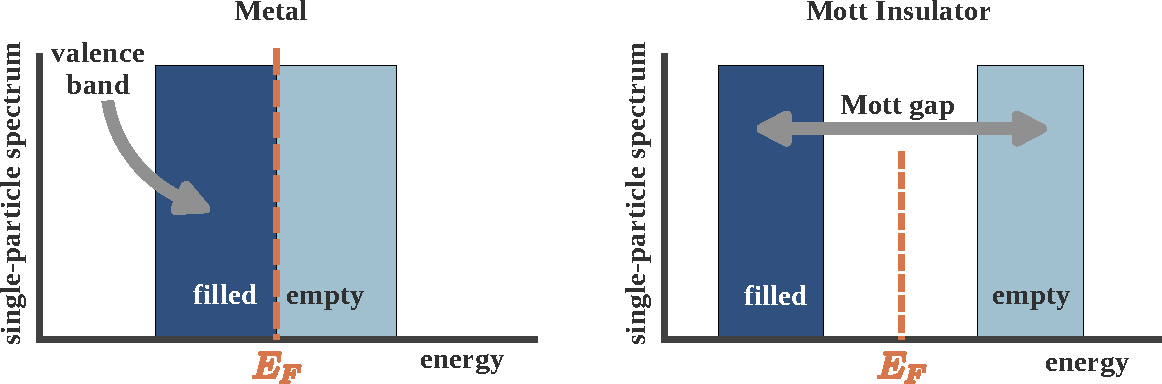
\includegraphics[width=\textwidth]{mottInsulator.pdf}
	\caption{}
	\label{mottInsulator}
\end{figure}

\section{Metal-insulator transition arising from strong correlation}
Initial attempts at explaining metal-insulator transitions was based on a non-interacting picture of electrons (through the work of Bethe, Sommerfeld, Bloch and Wilson among others); in such a picture, electronic bands can arise only from the scattering of electrons off the periodic lattice potential. One then distinguishes between metals and insulators at zero temperature by the position of the Fermi level \(E_F\) with respect to the bands: if \(E_F\) lies within a band gap, an integer number of bands will be completely filled and the system will be an insulator, whereas if \(E_F\) lies within one of the bands, the system will be a metal because there are vacant gapless excitations within the band. 

It was first pointed out by Boer and Verwey~\cite{Boer_1937} that certain insulators and semiconductors (such as nickel oxides) have a particle filling that, purely from band theory, would lead to partially filled bands. This poses a challenge because a partially filled band necessarily leads to a metallic phase (see Fig.~\ref{mottInsulator} (left)). The insulating behaviour of these materials therefore signals a fundamental limitation of single-particle band theory and points to a qualitatively different mechanism for electron localization---one driven by strong electron–electron interactions rather than by scattering from the lattice potential alone. This realization led to the concept of a Mott insulator, in which charge localization emerges as a genuine many-body effect despite the absence of a band gap in the non-interacting electronic structure. A very simple mechanism for this was put forth by Mott~\cite{Mott_1949,Mott1956,Mott961}: in the presence of a large local Coulomb repulsion cost \(U\) on a lattice site, the quantum states \(\ket{\Psi_1}\) in which the site is singly occupied get separated in energy from the states \(\ket{\Psi_2}\) where the site is doubly occupied by a gap of size \(U\); the former class of states \(\ket{\Psi_1}\) form the lower band (LB) while the latter \(\ket{\Psi_2}\) form the upper band (UB). If we now have a half-filled system (one electron per site), this electron will completely fill LB and leave UB vacant, leading to an insulating state (see Fig.~\ref{mottInsulator} (right)).

Given the above discussion, it is clear that a Mott insulator must involve a gap to charge excitations (excitations that add or remove an electron). It does not however determine the fate of the spin, orbital or other degrees of freedom. One scenario is when the spin or orbital degree of freedom undergoes spontaneous symmetry breaking into an ordered state; in the case of spin, this usually results in a superexchange interaction being generated and leads to an long-range ordered antiferromagnetic Neel state coexisting with the Mott state. Examples of such systems include vanadium sesquioxide V$_2$O$_3$ and its derivatives and the high-\(T_c\) cuprates (such as La$_2$CuO$_4$)~\cite{imada1998metal}. The other scenario is one where the spin degree of freedom retains its symmetry, and we end up with a quantum mechanically non-trivial entangled state (in order to quench the entropy). Examples of such states include quantum spin liquids~\cite{Isono2016}. Mott insulators without long-range order are of particular interest because of the possibility of topological order, fractional excitations, and novel metallic parent states.

A prototypical model for gaining theoretical understanding of Mott metal-insulator transitions on a lattice is the single-band Hubbard model~\cite{Anderson1959,hubbard1963electron,kanamori_1963,gutzwiller_1963}
\begin{equation}\begin{aligned}\label{hubbardModel}
	H = -t\sum_{\langle i,j \rangle , \sigma}(c^\dagger_{i,\sigma}c_{j,\sigma} + \text{h.c.}) - \frac{U}{2}\sum_i (n_{i, \uparrow} - n_{i, \downarrow})^2 - \mu N~.
\end{aligned}\end{equation}
The first term incorporates nearest-neighbour hopping on the lattice, while the second term introduces inter-electron repulsion when two electrons site on the same lattice site; in this way, the model incorporates the two competing tendencies of delocalisation and localisation that are responsible for the Mott MIT. The third term fixes the chemical potential and determines the filling of the lattice. Many of the materials that are studied for Mott MIT involve \(d-\)electrons that are five-fold degenerate, and these orbitals can hybridisation with ligand atoms. The Hubbard model avoids these complexities by focusing on only a single band that lies closest to the Fermi energy, and it is the states of this band that are described by the Hubbard model.

This leaves us with two channels for observing Mott MIT~\cite{imada1998metal}: (i) tuning the bandwidth, and (ii) tuning the filling. The former can be done, in experiments, by applying pressure. Filling is tuned by doping specific elements of a compound with elements of a different valence. The former is referred to as bandwidth-control metal-insulator transition, while the latter is called filling-control metal-insulator transition.

\section{Features of Mott metal-insulator transition}
\paragraph{Two complementary pictures of the Mott transition: Brinkman-Rice vs Mott-Hubbard.} Initial insights into the Mott MIT were obtained by Hubbard~\cite{hubbard1963electron}, thinking along lines similar to Mott. Within this picture, one starts from the insulating large \(U\) limit of the Hubbard model (eq.~\ref{hubbardModel}) (\(U \gg t\). We stay at half-filling for simplicity (\(\mu = 0\)). The large on-site repulsion leads to the formation of two bands at each site, the lower Hubbard band (LHB) associated with singly-occupied  states and the upper Hubbard band (UHB) associated with doubles and holes (states that incur a cost \(U\)). In the large \(U\) limit, these bands are well-separated, and the dynamics within the bands is a result of the motion of tightly bound holons and doubles (more on this later) that are generated because of the small but non-zero hopping probablity \(t\). As \(U/t\) is lowered, the bands come closer and a metal-insulator transition occurs at the critical value of \(U\) at which the gap vanishes. For lower \(U/t\), the bands overlap and we get a metal. This picture fails to provide an accurate description of the metal resulting from the melting of such a Mott insulator~\cite{georges1996}.

An alternative approach to the Mott MIT is due to Brinkman and Rice~\cite{brinkman_rice_1970}, where the authors applied Gutzwiller's variational method~\cite{Gutzwiller1965} to the half-filled Hubbard model. Gutzwiller's approach involves modifying, through variational factors, the hopping matrix elements that start from doubly occupied states, in order to reflect the electronic correlation at each site. By requiring that the number of doubly-occupied states vanish in the Mott insulating ground state, they obtained a critical value of the interaction strength. In the Brinkman-Rice scenario, therefore, the transition from the metal to the insulating phase occurs when the hopping matrix elements from the doubly-occupied to the singly-occupied states strictly vanishes. Note that in contrast to the Mott-Hubbard picture, this approach starts from a correlated Fermi liquid (renormalised due to the Gutzwiller factors). While it gives a better low-energy description of the correlated metal compared to the Mott-Hubbard picture, it fails to account for the high-energy physics, and treats the Mott insulator as a direct product state of local moments at each state (on account of the strictly zero hopping). This of course means that this method cannot explain antiferromagnetic superexchange processes in the Mott insulator~\cite{georges1996}.

\begin{figure}[!t]
	\centering
	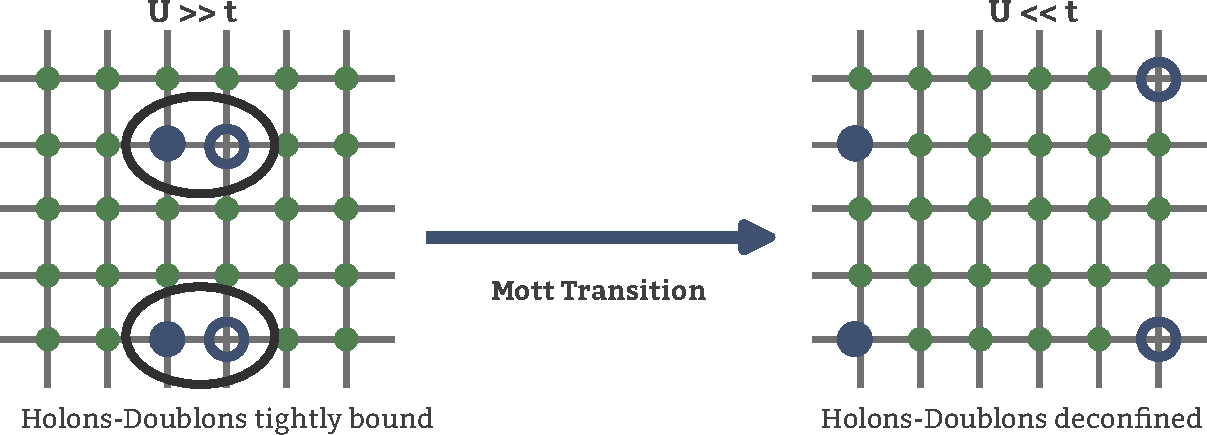
\includegraphics[width=\textwidth]{mottPicture.pdf}
	\caption{}
	\label{mottInsulator}
\end{figure}

\paragraph{Holon-doublon unbinding picture of the Mott MIT.} In 1949, Mott proposed a zero temperature explanation for a correlation-driven insulator and a mechanism for its transition into a metal in terms of the motion of holes and doubles in the background of a half-filled lattice. For \(U \ll t\) (strong correlation), the ground state predominantly involves lattice sites with a single electron. Hopping processes between two nearest-neighbour sites transfer an electron between them and create a pair of hole and double, but the pair remains tightly bound to each other. This is because moving the hole independently involves scattering processes that cross the Mott gap, and these processes are not allowed at \(T=0\). But without the independent motion of the hole (or double), there is no current, and the system is an insulator. 

As \(U/t\) is lowered, the gap closes and processes that transport the hole without transporting the double become gapless. This essentially means that the pair becomes deconfined, and the hole can be moved far away from the double. Current can then be passed by having the hole move through the lattice, and we get a metallic state. This leads to a picture of the Mott transition into a metal in terms of an unbinding of the hole-double bound states (excitons) that were present in the insulator.

There have been more quantitative studies of this mechanism. I list some of the relatively recent ones here. In~\cite{Prelovsek2015}, Prelovšek et al. studied the motion of holon-doublon pairs in a spin polarised background by rewriting the repulsive Hubbard model in terms of electrons as an attractive Hubbard model of holes and doubles. The model was treated using a BCS-like treatment, and the Mott transition was obtained when the binding energy for the hole-double condensate vanishes. To mark the deconfinement, they show that the approach to the transition from the insulating side is concomitant with an increase in the size of the pairs. Following a slave-boson treatment of holon-doublon unbinding, Zhou et al.~\cite{Zhou2014} show that the Mott transition from a paramagnetic metal to a Mott insulator on the half-field honeycomb and 2D square lattices occur through an intervening Slater insulator with coherent quasiparticles. In particular, their approach sheds light on the nature of the incoherent excitations in the Hubbard sidebands of the local spectral function. Finally, an older work by Watanabe et al.~\cite{Watanabe2006} studies the half-filled Hubbard model on an anisotropic triangular lattice using a Monte carlo method with a variational binding parameter between holons and doublons. Their approach reveals a first order Mott transition, along with robust \(d-\)wave superconductivity and short-range magnetic order.

\paragraph{Spectral features of the Mott transition.} One of the important diagnostics of the Mott metal-insulator transition is the spectrum for one-particle electron-like excitations, as expressed through the one-particle retarded Greens function \(G(\bm k,\sigma; t) = -i \theta(t)\langle \{c_{\bm k,\sigma}(t), c^\dagger_{\bm k, \sigma}\} \rangle \). In general, the presence of poles in the Green function at the Fermi energy and in its neighbourhood imply the existence of gapless excitations and hence a metallic phase. It turns out that this statement is equivalent to Luttinger's theorem,
\begin{equation}\begin{aligned}
	\frac{N}{V} = 2\int_{G(0,\bm k)>0}\frac{d\bm k}{(2\pi)^3}~,
\end{aligned}\end{equation}
which states that the particle density in a metal is equal to the number of states in the Fermi volume. As clarified in the equation, the Fermi volume is defined as the region of \(k-\)space where the Greens function is positive at \(\omega=0\).

In a Mott insulator, strong correlations lead to the destruction of electronic excitations around \(\omega=0\). This results in the Greens function poles transmuting into zeros. This is also tracked by analogous changes in the electronic self-energy \(\Sigma({\bm k};\omega)\); Greens function zeros leads to a Mott pole at \(\omega=0\) in \(\Sigma({\bm k};\omega)\). The points in \(k-\)space where \(\Sigma({\bm k};0)\) vanishes is called a Luttinger surface. The Mott metal-insulator transition is therefore about the topological change of a Fermi surface (surface of Greens function poles) into a Luttinger surface (surface of self-energy poles).

As discussed earlier, the appearance of Greens function zeros at \(\omega=0\) leads to the formation of a charge gap that freezes one-particle low-energy excitations. The spectrum gets redistributed into two bands on either side of the gap, the upper and lower Hubbard bands. In the ground state, the lower band is obviously filled while the upper band is empty. Bands of a Mott insulator formed from electronic correlation differ from those formed due to one-particle scattering in a particular way: dynamical spectral weight transfer. Unlike a band insulator, the bands of a Mott insulator are not rigid; tuning the lattice filling results in a continuous transfer of states from one band to another. 

The non-rigidity of the bands can be seen most easily from the atomic limit (\(t=0\)) of the Hubbard model (eq.~\ref{hubbardModel}). The local retarded Greens function at an arbitrary site \(i\) can be obtained using the equation of motion approach. The final result is~\cite{phillips2012advanced}
\begin{equation}\begin{aligned}
G_R(i; \omega) = \frac{1 + x}{\omega + \mu + U/2} + \frac{1 - x}{\omega + \mu - U/2}~,
\end{aligned}\end{equation}
where \(x = 1 - \sum_\sigma\langle n_{i\sigma} \rangle \) is the average number of holes at any site. The spectral weight for the two poles makes it clear that the lower band has \(1+x\) number of states while the upper band has \(1-x\) states. Changing the number of states in the lower band (by tuning \(\mu\) and hence \(x\)) also changes those in the upper band. For example, by adding \(0.1\) holes per site to the lower band, the spectral weight in the upper band decreases by the same amount. This is the non-rigidity of the bands mentioned previously.

\section{Preliminary Insights Into Mottness: The Baskaran-Hatsugai-Kohmoto model}
\begin{figure}[!t]
	\centering
	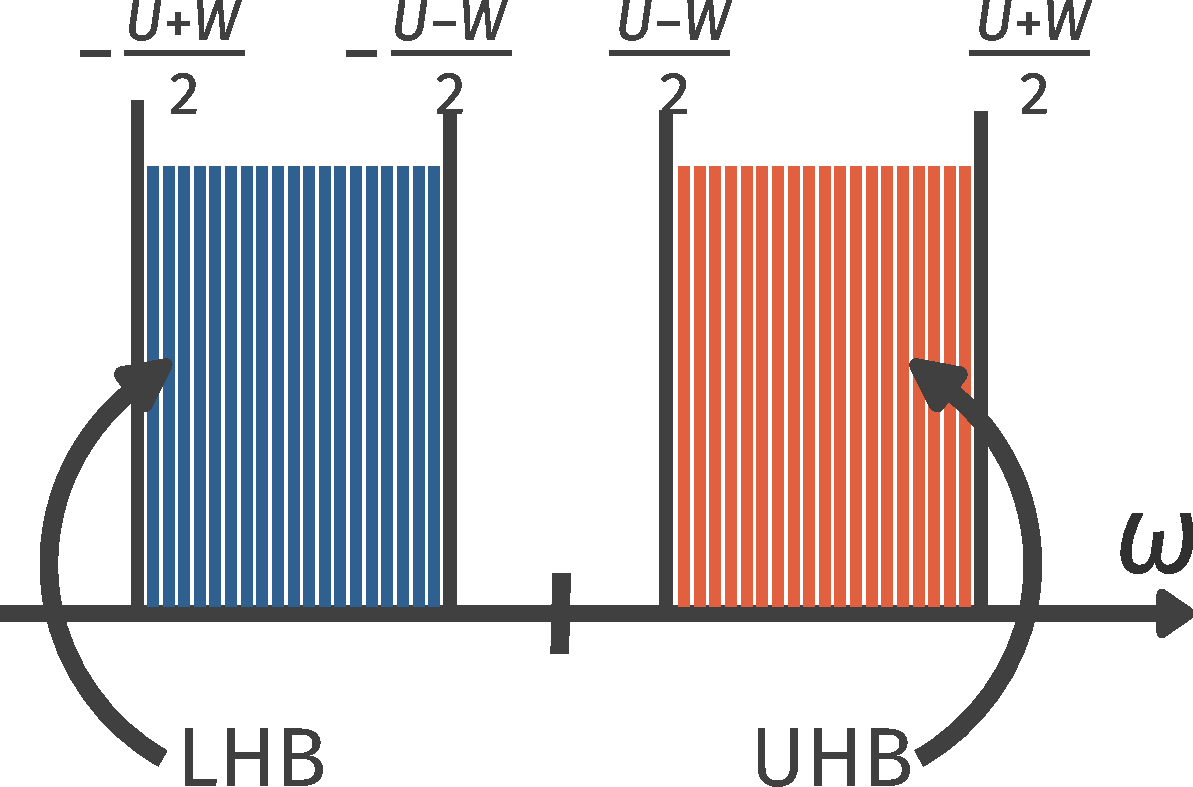
\includegraphics[width=0.48\textwidth]{insulator.pdf}
	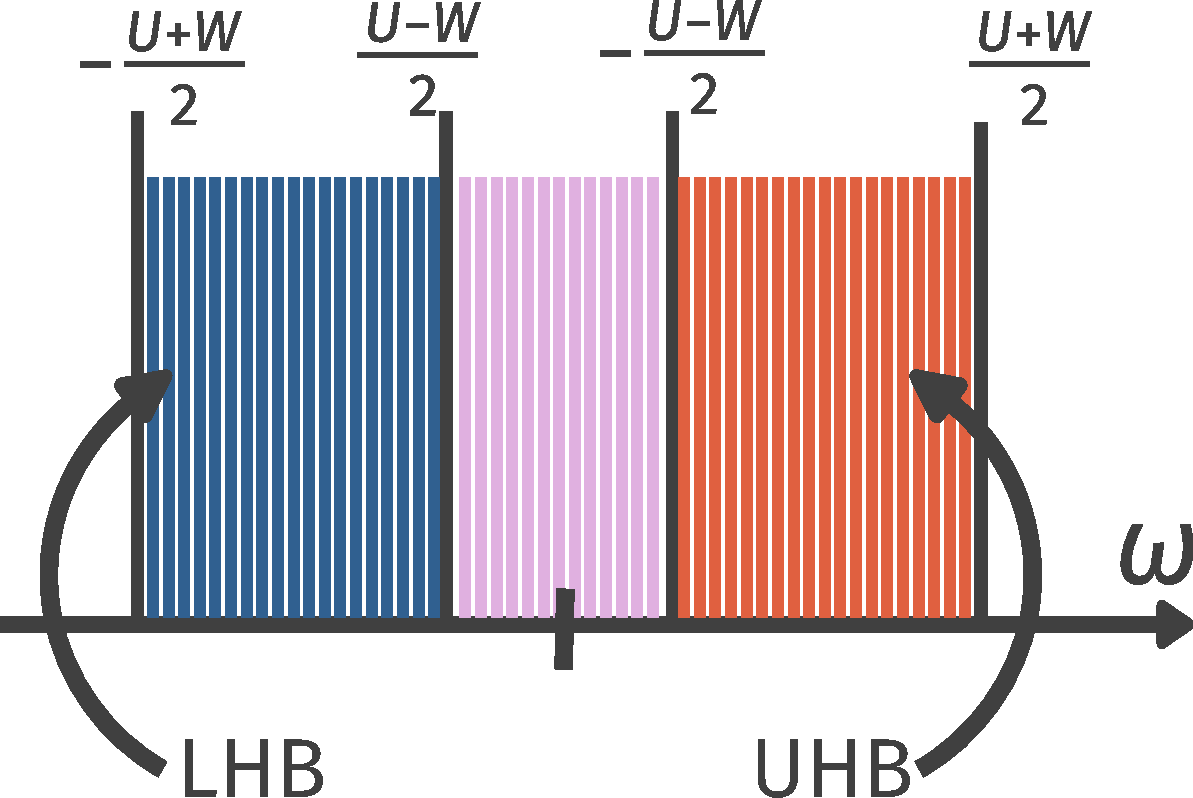
\includegraphics[width=0.48\textwidth]{metal.pdf}
	\caption{}
	\label{HKM-phases}
\end{figure}
The Baskaran-Hatsugai-Kohmoto model~\cite{Baskaran1991,Hatsugai1992} introduced independently in 1991 and 1992 is an exactly solvable model of electronic correlation that displays a transition from a metallic phase to a Mott insulator. While it's solvability offers an instructive method for studying Mott transition, the infinitely long-ranged nature of its interaction makes it tricky to apply these conclusions to realistic materials.

At half-filling, the model is defined by the following Hamiltonian:
\begin{equation}\begin{aligned}
	H_\text{BHK}= \sum_{\bf k,\sigma}\epsilon({\bf k}) n_{\bf k,\sigma} - \frac{U}{2}\sum_{\bf k}(n_{\bf k, \uparrow} - n_{\bf k,\downarrow})^2~.
\end{aligned}\end{equation}
Clearly the model is diagonal in momentum-space; the Hamiltonian splits up into commuting \(4\times 4\) blocks for every point \(\bf k\):
\begin{equation}\begin{aligned}
	H_\text{BHK} = \sum_{\bf k}H({\bf k}), \quad H({\bf k}) = \epsilon({\bf k}) \sum_\sigma n_{\bf k,\sigma} - \frac{U}{2}(n_{\bf k, \uparrow} - n_{\bf k,\downarrow})^2~.
\end{aligned}\end{equation}
The vacant eigenstate \(\ket{0}\) of \(H({\bf k})\) has zero energy (\(E_0 = 0\)), the two singly-occupied states \(\ket{\uparrow}\) and \(\ket{\downarrow}\) have energy \(E_1 = \epsilon({\bf k}) - U/2\) and the doubly-occupied state \(\ket{\uparrow, \downarrow}\) has energy \(E_2 = 2\epsilon({\bf k})\). This leads to two possible single-particle excitations -- one for adding an electron on the vacant state: (\(\Delta_1 = E_1 - E_0 = \epsilon({\bf k}) - U/2\), the other for adding an additional electron on a singly-occupied state: \(\Delta_2 = E_2 - E_1 = \epsilon({\bf k}) + U/2\). 

Upon combining states from other \(k-\)modes, these isolated excitations broaden into bands around \(\pm U/2\) because of the continuum of values available to \(\epsilon({\bf k})\). For large enough \(U\) (compared to the non-interacting bandwidth \(W\)), these bands remain well-separated in energy (Fig.~\ref{HKM-phases} left), forming lower and upper Hubbard bands. The half-filled system results in the lower band being completely filled and the upper band empty, leading to a Mott insulator. The states within this band are all singly-occupied (per \(k-\)state). Upon lowering the correlation strength \(U\), the bands touch each other at the critical value of \(U_c = W\) (obtained by equating the top of the lower band to the bottom of the upper band). For lower values of \(U\), the system is a metal due to the presence of gapless excitations within the combined band (Fig.~\ref{HKM-phases} right). This therefore provides a simple demonstration of a correlation-driven Mott metal-insulator transition.

\section{Strong local correlations and auxiliary models}
\subsection{Introduction to the auxiliary model approach}
One of the main results obtained within this thesis is the development of a formalism to study the more realistic case of finite-dimensional interacting models by using appropriately chosen impurity models as auxiliary models. The key to an {\it auxiliary model method} is to construct an appropriate auxiliary model that while being tractable captures some essential property of the full lattice model~\cite{martin_2016}. This involves separating the complete degrees of freedom into a system part (\(H_S\)) which one treats exactly and the rest of the system (\(H_R\)) that one might simplify in order to be able to solve the problem. The non-trivial nature of the problem arises of course from the hybridisation \(H_{SR}\) between the system and the bath:
\begin{equation}\begin{aligned}
	{H} &= \begin{bmatrix} & {H}_{R} && {H}_{RS} & \\ & {H}_{RS}^* && {H}_{S} & \end{bmatrix}~.
\end{aligned}\end{equation}

This separation can always be done exactly, if one does not care about tractability. For example, one can take the Hubbard model that describes electrons hopping on a lattice and interacting when two electrons reside on the same lattice site:
\begin{equation}\begin{aligned}
	H_\text{hub} = -t\sum_{\langle i,j \rangle,\sigma }(c^\dagger_{i,\sigma}c_{j,\sigma} + \text{h.c.}) + U\sum_{i}n_{i \uparrow}n_{i \downarrow}~,
\end{aligned}\end{equation}
and separate this into parts, the system being the local orbitals of a specific site \(l\) and the rest of the system being all the other sites:
\begin{equation}\begin{aligned}
	H_S = U n_{l \uparrow} n_{l \downarrow},~~ H_R = -t\sum_{\langle i,j \rangle,\sigma }^\prime(c^\dagger_{i,\sigma}c_{j,\sigma} + \text{h.c.}) + U\sum_{i}^\prime n_{i \uparrow}n_{i \downarrow},~~ H_{SR} + H_{RS} = -t\sum_{i,\sigma} (c^\dagger_{l,\sigma}c_{i,\sigma} + \text{h.c.})~,
\end{aligned}\end{equation}
where the primed summation is carried out over all nearest-neighbour pairs that do not involve \(l\) and the summation in \(H_{SR} + H_{RS}\) is over all sites adjacent to \(l\).

The smaller system \(H_S\) (often called the {\it cluster}) is typically chosen such that its eigenstates are known exactly. Progress is then made by choosing a simpler form for \(H_R\) and its coupling \(H_{RS}\) with the smaller system. This combination of the cluster and the simpler bath is then called the \textit{auxiliary system}.
A tractable auxiliary system for the Hubbard model is the single-impurity Anderson model (SIAM); the correlated impurity site represents the set of local orbitals of any given site, while the conduction bath represents the rest of the lattice sites in an approximate fashion.  Such a construction is shown in fig.~\ref{cluster-bath}.
\begin{figure}[!htb]
	\centering
    
\includegraphics[width=0.9\textwidth]{clusterBath.pdf}
	\caption{\textit{Left}: Full Hubbard model lattice with onsite repulsion $U^H$ on all sites and hopping between nearest neighbour sites with strength $t^H$. \textit{Right}: Extraction of the auxiliary (cluster+bath) system from the full lattice. The central site on left becomes the impurity site (red) on the right (with an onsite repulsion $\epsilon_d$), while the rest of the $N-1$ sites on the left form a conduction bath (green circles) (with dispersion $\epsilon_k$ and correlation modelled by the self-energy $\Sigma_k(\omega)$) that hybridizes with the impurity through the coupling $V$.}
	\label{cluster-bath}
\end{figure}

It should be noted that any reasonable choice of the cluster and bath would break the translational symmetry of the full model: To allow computing quantities, one would need to make the bath (which is a much larger system) simpler than the cluster (which is a single site). This distinction breaks the translational symmetry of the Hubbard model. As a result, calculations that make use of the translation symmetry of the full model (such as \(k-\)space objects) will require a periodisation operation of an auxiliary model quantity.
\subsection{Correspondence between impurity and lattice models in $d=\infty$}

Dynamical Mean-Field Theory (DMFT) provides a nonperturbative framework for treating strong local electronic correlations in lattice models by mapping them onto a self-consistent quantum impurity problem \cite{Metzner1989,Georges1996}. The central idea of DMFT is that in the limit of infinite spatial dimension, or equivalently infinite coordination number, the electronic self-energy becomes purely local while retaining its full dynamical (frequency-dependent) structure. As a result, the many-body lattice problem reduces to an effective single-site problem embedded in a self-consistently determined bath, capturing local quantum fluctuations exactly while neglecting nonlocal correlations. DMFT has become a cornerstone of modern correlated-electron theory, successfully describing Mott metal--insulator transitions, quasiparticle formation, and spectral weight transfer in Hubbard-like models \cite{Georges1996,Kotliar2004,Georges2004}.

In order to motivate the impurity model-lattice model mapping inherited by DMFT, we first recall the textbook example of classical mean-field theory. Mean-field theory provides one of the earliest and most instructive examples of controlled approximations in many-body physics. In its classical incarnation, exemplified by the Ising model,
\begin{equation}
	H_{\mathrm{Ising}} = - \sum_{i\neq j} J_{ij} S_i S_j - h \sum_i S_i = -\sum_i S_i(h + \sum_{j \neq i}J_{ij}S_j),
\end{equation}
mean-field theory proceeds by replacing the interaction between a given spin and its neighbors by an {\it effective static field} proportional to the average magnetization. Writing
\(
S_j = \langle S_j \rangle + \delta S_j
\)
and neglecting quadratic fluctuations and constant parts, one obtains an {\it auxiliary problem} in the form of a mean-field Hamiltonian
\begin{equation}\begin{aligned}
	H^{(\text{MF})}_{\mathrm{Ising}} = - \sum_{i} (h + h_\text{MF}(i))S_i~,
\end{aligned}\end{equation}
where the mean-field \(h_\text{MF}\) comes out to be
\begin{equation}\begin{aligned}\label{mean-field}
	h_\text{MF}(i) = \sum_{j \neq i}2 \langle S_j \rangle J_{ij}~.
\end{aligned}\end{equation}
The above approach assumes two things: (i) the presence of a non-zero {\it order parameter} \(m_j = \langle S_j \rangle \) (in this case, a non-zero magnetisation), and (ii) the smallness of the fluctuations \(S_j - \langle S_j \rangle\). The mean-field Hamiltonian can be used to compute the partition function (at inverse temperature \(\beta\)) and hence the magnetisation at a site \(i\) of the lattice:
\begin{equation}\begin{aligned}\label{magnetisation}
	m_i = \tanh(\beta(h_\text{MF}(i) + h)) = \tanh(\beta \sum_{j \neq i}2 m_j J_{ij} + \beta h)~.
\end{aligned}\end{equation}

The problem hasn't yet been solved of course; one needs to determine the appropriate value of \(m_j\). We therefore need an additional equation; this is provided by the so-called {\it self-consistency condition}. The translation invariance of the lattice ensures that the magnetisation must be uniform across sites \(i\) and \(j\). This allows us to replace \(m_j\) with \(m_i\) in the above equation:
\begin{equation}
	m_i = \tanh(\beta m_i\sum_{j \neq i}2 J_{ij} + \beta h)~.
\end{equation}
This equation can be solved numerically to obtain the uniform magnetisation \(m_i = m\).
The mean-field approximation becomes exact in the limit of large coordination, where fluctuations are suppressed  and spatial correlations beyond a single site vanish.

An equivalent way of framing the self-consistency equation is to equate the mean-fields on different lattice sites. Combining eqs.~\ref{magnetisation} and \ref{mean-field}, we have
\begin{equation}\begin{aligned}
	h_\text{MF}(i) = \sum_{j \neq i}2 m_j J_{ij} = \sum_{j \neq i}2 \tanh(\beta(h_\text{MF}(j) + h)) J_{ij}~.
\end{aligned}\end{equation}
The equation in terms of \(h_\text{MF}(i)\) and \(h_\text{MF}(j)\) can again be solved numerically by claiming that the mean-field has to be uniform across all the sites owing to translation invariance. This form of the self-consistency requirement (in terms of the field) will be useful to us in the upcoming discussion.


The essential feature of classical mean-field theory is therefore the replacement of a many-body problem by an effective \emph{single-site} problem embedded in a self-consistently determined environment. Quantum lattice models admit a closely analogous construction, but with an important conceptual difference: while the classical mean field is static, quantum fluctuations necessarily introduce a tower of excited states that allow for temporal dynamics. This observation underlies the formulation of dynamical mean-field theory (DMFT), which may be viewed as the natural quantum generalization of classical mean-field theory \cite{metzner_volhardt_1989,georges1996}.

Similar to the previous case of the Ising model, we will now derive the self-consistency equation for a quantum model. Consider an interacting fermionic lattice Hamiltonian, such as the Hubbard model:
\begin{equation}
H = -\sum_{ij\sigma} t_{ij} c_{i\sigma}^\dagger c_{j\sigma}
+ U \sum_i n_{i\uparrow} n_{i\downarrow},
\end{equation}
defined on a lattice with coordination number \(z\). 
% To obtain a nontrivial limit as \(z \to \infty\), the hopping amplitudes are scaled as
% \begin{equation}
% t_{ij} = \frac{t^\ast}{\sqrt{z}},
% \end{equation}
% which ensures a finite kinetic energy per site \cite{MetznerVollhardt1989}.

% In this limit, it can be shown diagrammatically that all nonlocal contributions to the self-energy vanish as inverse powers of \(z\), while local diagrams remain finite. As a result, the exact self-energy becomes purely local,
% \begin{equation}
% \Sigma_{ij}(\omega) = \delta_{ij}\,\Sigma(\omega),
% \end{equation}
% though it retains its full dynamical (frequency-dependent) character \cite{MetznerVollhardt1989,Georges1996}.

The point of this exercise is to calculate the interacting self-energy \(\Sigma_k(\omega)\) for the fermions. This therefore acts as an ``order parameter" and plays the same role as the local magnetisation in the previous exercise. The self-energy defines the interacting \(k\)-space Green's function for a translation-invariant problem:
\begin{equation}
	G_{\mathbf{k}}(\omega) = \frac{1}{\omega - \varepsilon_{\mathbf{k}} - \Sigma_{\mathbf{k}}(\omega)},
\end{equation}
where \(\varepsilon_{\mathbf{k}}\) denotes the noninteracting dispersion, and a real-space local Green's function, obtained by summing over momentum:
\begin{equation}\label{eq:localG}
G_{\text{loc}}(\omega) = \sum_{\mathbf{k}} \frac{1}{\omega - \varepsilon_{\mathbf{k}} - \Sigma_{\mathbf{k}}(\omega)}.
\end{equation}

Similar to the earlier exercise, we need to apply a mean-field decoupling to drop certain fluctuations and obtain a similar effective problem. In the context of interacting electrons, such a decoupling is obtained in the limit of infinite dimensionality or coordination number, where the self-energy becomes \(k-\)independent~\cite{metzner_volhardt_1989}:
\begin{equation}\begin{aligned}
	\Sigma_{\mathbf{k}}(\omega) = \Sigma_\text{loc}(\omega), \text{ or (equivalently) }~ \Sigma_{ij}(\omega) = \delta_{ij}\Sigma_\text{loc}(\omega)~.
\end{aligned}\end{equation}
The mean-field decoupling here therefore corresponds to ignoring spatial fluctuations of the one-particle self-energy, and leads to a local Greens function that is directly connected to the local self-energy:
\begin{equation}\begin{aligned}
G_{\text{loc}}(\omega) = \sum_{\mathbf{k}} \frac{1}{\omega - \varepsilon_{\mathbf{k}} - \Sigma_\text{loc}(\omega)}.
\end{aligned}\end{equation}
It turns out that a local Greens function connected to a local self-energy also defines a quantum impurity problem describing the dynamics of a single correlated site with the other environment sites integrated out:
\begin{equation}\label{effAction}
	S_{\text{imp}} = -\int_0^\beta d\tau d\tau'\,c^\dagger(\tau)\,G_\text{MF}^{-1}(\tau-\tau')\,c(\tau') + U \int_0^\beta d\tau\, n_\uparrow(\tau) n_\downarrow(\tau).
\end{equation}
This acts as an auxiliary problem for the more complete problem locally interacting electrons on a lattice. The non-interacting Greens function \(G_\text{MF}\) is as of now unknown, and defines the environment of the impurity site and comprises the dynamics of the sites that have been integrated out. Such an impurity problem is solvable, and the impurity Green's function is given by
\begin{equation}
	G_{\text{imp}}(\omega) = \frac{1}{G_\text{MF}^{-1}(\omega) - \Sigma_\text{imp}(\omega)},
\end{equation}

The first term in eq.~\ref{effAction} is therefore what makes this problem dynamical -- it represents the probability of electrons hopping into and out of the impurity site, and leads to fluctuations of its occupancy. We can make the identification of the Greens function \(G_\text{MF}\) as the {\it mean-field} encountered in the previous example. More specifically, \(G_\text{MF}\) acts as a ``field" because it is obtained by integrating out the other sites on the lattice, and it acts on the impurity site by affecting its dynamics.

The complete set of equations for the solving such a dynamical mean-field problem is finally obtained by equating the impurity local Greens function \(G_\text{imp}\) to the lattice local Greens function \(G_\text{loc}\). As discussed earlier, such a solution exists in an exact fashion only in the limit of infinite dimensions, as long as the correct \(G_\text{MF}\) can be found. In order to find the appropriate \(G_\text{MF}\) that allows equating the impurity model Greens function to a lattice mode Greens function, we require an additional equation: the self-consistency condition. Similar to the case of the Ising model, we require that \(G_\text{MF}\) be equal to \(G_\text{loc}\), owing to translation invariance. The full set of coupled DMFT equations is
\begin{equation}\begin{aligned}
	G_\text{MF}	&= G_\text{loc},\\
	\Sigma_\text{imp}(\omega) &= G_\text{MF}^{-1}(\omega) - G^{-1}_{\text{imp}}(\omega),\\
	\Sigma_\text{loc}(\omega) &= \Sigma_\text{imp}(\omega),\\
	G_{\text{loc}}(\omega) &= \sum_{\mathbf{k}} \frac{1}{\omega - \varepsilon_{\mathbf{k}} - \Sigma_\text{loc}(\omega)}.
\end{aligned}\end{equation}
\begin{itemize}
	\item The first equation is equivalent to the feature in the previous exercise where we equated the mean-fields on \(i\) and \(j\).
	\item The second equation is equivalent to computing, in the previous exercise, the magnetisation on the \(j^\text{th}\) site from the partition function.
	\item The third equation is the essential mean-field approximation, where we equate the self-energy of the simpler decoupled problem to that of the more complete lattice problem and is justified in the limit of infinite dimensions.
	\item The fourth equation is equivalent, in the previous exercise, to using the computed ``magnetisation" of site \(j\) in the second step to further compute the mean-field at site \(i\).
\end{itemize}

In direct analogy with classical mean-field theory, DMFT replaces a lattice model by an effective single-site problem embedded in a self-consistent environment. The crucial distinction is that the mean field is now dynamical rather than static, encoding quantum fluctuations exactly while neglecting spatial correlations. Importantly, this demonstrates the importance of quantum impurity models in investigating correlated lattice models, particularly in the presence of strong local interactions. This is because the effects of local correlations are captured exactly by such an auxiliary model mapping.

\subsection{Examples of strongly correlated materials}
As discussed in the previous section, the route to studying lattice problems via quantum impurity models makes most sense for models with strong local correlations. 

\paragraph{Transition Metal Oxides (TMOs)}
Transition Metal Oxides (TMOs) are defined chemically by the presence of partially filled $d$-shells in transition metals (e.g., Cu$^{2+}$, Mn$^{3+}$, V$^{4+}$) coordinated by oxygen ligands. The physics of TMOs is governed by the competition between the kinetic energy hopping amplitude $t$ and the on-site Coulomb repulsion $U$; due to the small overlap between the localised \(d-\)orbitals, the \(d-\)electrons can delocalise only by hopping onto the ligand atoms. According to the Zaanen-Sawatzky-Allen (ZSA) classification scheme~\cite{Zaanen1985}, these materials are categorized as either Mott-Hubbard insulators, where the charge gap is determined by the $d$-$d$ Coulomb interaction ($E_g \approx U$), or charge-transfer insulators, where the gap is dictated by the energy difference between the oxygen $p$-band and the metal $d$-band. These derive from considerations of several factors, such as crystal field splitting, arrangement of atoms and lattice symmetries. 

For example, in the case of octahedral symmetry, repulsion from the surrounding atoms leads to the raising of energy of the \(d_{x^2 - y^2}\) and \(d_{3z^2-r^2}\) orbitals forming the \(e_g\) doublet, while the other three orbitals (\(d_{xy}, d_{yz}\) and \(d_{zx}\)) form the \(t_{2g}\) multiplet. For the heavier TMOs (Ti, V, Cr...), the Fermi level lies within \(e_{g}\). The increased positive nuclear charge (compared to the lighter elements) lowers the energy of the \(d-\)orbitals and brings them closer to the \(p-\)orbitals, reducing the charge transfer energy \(\Delta = \varepsilon_d - \varepsilon_p\) of transporting an electron from a \(d-\)state to a \(p-\)state, compared to the \(d-\)level repulsion \(U\) (\(|\Delta| < U\)). Geometric reasons (the \(e_g\) orbitals point towards the \(p-\)orbitals) also enhance the hybridisation between \(d-\) and \(p-\)orbitals in such materials. If \(\Delta\) becomes larger than the bandwidth, we obtain a {\it charge-transfer insulator}, where the charge gap is decided by \(\Delta\). In the lighter TMOs, the Fermi level passes through \(t_{2g}\), and because they point away from the \(p-\)orbitals, the hybridisation is weaker. Moreover, the reduced positive nuclear charge leads to an increased \(\Delta > U\); a \(U\) greater than the bandwidth leads to what's called a {\it Mott-Hubbard insulator}.

Experimental studies of transition metal oxides (TMOs) have established metal–insulator transitions (MITs) as a defining consequence of strong electronic correlations in systems with partially filled (d)-electron shells \cite{Imada1998,mcwhan1969}. Early experiments on vanadates such as $V_2O_3$ characterised pressure-driven MITs through the pressure- and temperature-dependent conductivity as well as an anomalous enhancement of the optical conductivity\cite{Limelette2003,Rozenberg1995,Qazilbash2007}. Copper oxides constitute the most extensively studied class of correlated TMOs and provide a canonical example of a doping-driven MIT. Transport measurements on parent compounds such as $La_2CuO_4$ establish a robust insulating state, while carrier doping leads to anomalous metallic behavior characterized by linear-in-temperature resistivity and unconventional superconductivity\cite{Takagi1992,Ando2004,Lemberger2011}. Such metal-insulator transition is also reported from angle-resolved photoemission spectroscopy (ARPES) measurements in doped $La_2CuO_4$ and $Bi_2Sr_2CaCu_2O_8$, along with the emergence of pseudogap near the antinodes at high temperatures and a hole-to-electronlike Fermi surface reconstruction\cite{Damascelli2003,Sobota2021,Vishik_2018}. Nickelates ($LaNiO_2$, $La_3Ni_2O_7$, $La_4Ni_3O_{10}$, etc) exhibit related but distinct experimental signatures. With \(Ni^+\) sharing the same \(3d^9\) valence configuration as \(Cu^{2+}\) in the cuprate superconductors, these materials also display superconductivity, although the mechanism in the nicklelates is different due to the strong coupling between the layers~\cite{Medarde_1997,Wang2025}. The optimal doped regime in thin films shows strange metal behaviour, while infinite-layer nickelates show the absence of long-range antiferromagnetic order~\cite{Puphal2026}.

\paragraph{Transition Metal Dichalcogenides}
Transition Metal Dichalcogenides (TMDs) are layered van der Waals materials with the stoichiometry $MX_2$, where $M$ is a transition metal (e.g., Mo, W) and $X$ is a chalcogen (e.g. S, Se, Te)~\cite{Manzeli2017,Joseph2023}. Recent interest has focused on the interplay between strong spin-orbit coupling (SOC), electronic correlations and direct bandgap -- properties that make them particularly useful for electronic applications, spintronics and DNA sequencing. Layered TMDs have the structure \(X-M-X\), with the transition metal sandwiched between two hexagonal planes of chalcogenides. Different combinations of the metals with the chalcogens lead to widely varying structures and electronic properties in TMDs. Experimental studies show that metal--insulator transitions (MITs) in TMDs are commonly intertwined with charge density wave (CDW) formation rather than arising from purely on-site Coulomb localization~\cite{Wilson1974PRL,Wilson2001}. In prototypical compounds such as 1T-TaS$_2$, ARPES and transport measurements reveal fluctuating magnetic order parameters in the Mott state and a transition to superconductivity driven by pressure \cite{Fazekas1979,Perfetti2005,Sipos2008}. Scanning tunnelling microscope (STM) pulses have been successfully used to manipulate the metal–insulator transition of 1T-TaS2, demonstrating the macroscopic controllability of the Mott phase\cite{Cho2016}.

ARPES measurements in 2H-NbSe$_2$ and 2H-TaSe$_2$ partial gapping of the Fermi surface restricted to nested momentum regions and a temperature-dependent pseudogap similar to the cuprates\cite{Borisenko2008,Borisenko2009}. This is further supported by optical conductivity experiments that show spectral weight in the midinfrared region along with a low-frequency Drude contribution~\cite{Vescoli1998}. Transport measurements on single crystals of TaSe$_2$ reveal that disorder enhances superconductivity by suppressing other competing orders such as CDW~\cite{Li2017}. Collectively, these experimental results establish TMDs as a distinct class of correlated materials in which reduced dimensionality, band narrowing, and lattice reconstruction cooperate to produce metal--insulator behavior beyond conventional band theory.

\paragraph{Iron-Based Superconductors}
The iron-based superconductors (FeSCs), discovered in 2008, constitute a broad family of layered materials that share a common structure: a layer of iron atoms joined by tetrahedrally coordinated pnictogen (P, As) or chalcogen (S, Se, Te) anions arranged in a stacked sequence; the layers are separated by alkali, alkaline-earth or rare-earth and oxygen/fluorine ‘blocking layers’\cite{kamihara2008,Paglione2010,Hirschfeld2011,stewart2011}. Doping or applying external pressure reveals coupled antiferromagnetic and structural transitions along with superconducting and nematic orders~\cite{Johnston2010,Kasahara2012,Fernandes2014}. Electrical resistivity measurements in the neighbourhood of the quantum critical point show a crossover from a bad-metal behavior (\(T-\)linear resistivity)  to a Fermi liquid behaviour (\(T^2-\)resistivity) \cite{Analytis2014}. Optical conductivity measurements indicate point to intermediate-to-strong electronic correlations \cite{Qazilbash2009}.

ARPES measurements reveal a \(k-\)dependent superconducting gap and de Haas-van Alphen measurements indicate substantial quasiparticle mass enhancements, shedding more light on the correlated nature of the material\cite{Shishido2010,terashima2009}. Strain-tuning measurements of the nematic susceptibility, and differential elastoresistance measurements have provided compelling evidence for the nematic transition and its surrounding fluctuations being the cause of the structural transition as well as the superconductivity\cite{Chu2012,Kuo2016}. Neutron scattering and NMR measurements further reveal persistent low-energy spin fluctuations across wide regions of the phase diagram, supporting scenarios in which unconventional superconductivity emerges from the interplay of magnetic, orbital, and nematic degrees of freedom \cite{Inosov2010,Chubukov2012}.

\paragraph{Heavy-Fermion / Kondo-Lattice Systems}
Heavy-fermion materials are a class of strongly correlated electron systems typically realized in intermetallic compounds of rare earth metals (such as Ce, Sm and Yb) and actinides (such as U, Np and Pu), where localized $f$ electrons hybridize with itinerant conduction bands \cite{Stewart1984,Wirth2016}. At high temperatures, these systems exhibit local-moment behavior governed by Curie--Weiss susceptibilities and incoherent transport, while at low temperatures the Kondo effect leads to the formation of a coherent many-body state with extremely large quasiparticle effective masses \cite{hewson1993}. Experimentally, this crossover is most clearly manifested in transport and thermodynamic measurements: the electrical resistivity shows a characteristic maximum followed by a rapid drop signaling the onset of coherence, while the linear specific heat coefficient $\gamma=C/T$ reaches values orders of magnitude larger than in conventional metals, directly reflecting the heavy quasiparticle mass \cite{Lohneysen2007}.

A defining feature of heavy-fermion materials is their proximity to magnetic quantum phase transitions, which can be accessed experimentally by pressure, chemical substitution, or magnetic field~\cite{Gegenwart2008}. Near such quantum critical points (QCPs), transport measurements reveal pronounced non-Fermi-liquid behavior ($T-$linear resistivity) and a vanishing Hall response, along with a divergent effective quasiparticle mass as the transition is approached~\cite{Custers2003,Paschen2004}; these are all indications of the breakdown of electronic excitations near the transition. Neutron scattering experiments provide direct evidence for spin fluctuations down to very low temperatures, interplaying with the itinerant electrons at the QCP and potentially driving the superconducting transition~\cite{Schroder2000,Stockert2011}. Quantum oscillation measurements through de Haas–van Alphen experiments further demonstrate Fermi surface reconstruction across the quantum critical point, highlighting the drastic change in Fermi volume~\cite{Shishido2005}. Together, these experimental observations establish heavy-fermion compounds as paradigmatic systems in which strong local correlations, hybridization-driven coherence, and quantum critical fluctuations conspire to produce emergent low-energy quasiparticles and unconventional metallic behavior~\cite{Si2010}.

\section{Phenomenology of the Anderson impurity model}
Within this thesis, we have developed an auxiliary model approach that combines the physics of quantum impurity models with a manybody version of Bloch's theorem to investigate interacting fermionic lattice models. This is motivated by the relative ease in solving impurity models and transparency afforded by such solutions. We now review the phenomenology of some of these impurity models and point out how the various impurity features affect the physics of the lattice models.

The single-impurity Anderson model describes the dynamics of a system of non-interacting itinerant electrons \((c_{k,\sigma})\) hybridising with a localised correlated impurity orbital (\(d_\sigma\))~\cite{Anderson1959}:
\begin{equation}\begin{aligned}
	H_\text{AIM} = \sum_{k,\sigma}\epsilon_k n_{k,\sigma} + \sum_{k,\sigma}V_k(c^\dagger_{k,\sigma}d_\sigma + \text{h.c.}) + \epsilon_d \sum_\sigma n_{d\sigma} + Un_{d \uparrow} n_{d \downarrow}~.
\end{aligned}\end{equation}
\(V_k\) controls the hybridisation strength, and \(\epsilon_d\) and \(U\) control the onsite energy and local correlation respectively of the impurity site. In the limit of large \(U\), the impurity dynamics gets projected onto its spin states, and the model then describes the scattering of non-interacting electrons off magnetic impurities, through the Kondo model:
\begin{equation}\begin{aligned}
	H_\text{Kondo} = \sum_{k,\sigma}\epsilon_k n_{k,\sigma} + J \sum_{k_1,k_2}\sum_{\alpha,\beta}\vec{S}_d \cdot \vec{\sigma}_{\alpha,\beta}c^\dagger_{k_1,\alpha}c_{k_2,\beta}~,
\end{aligned}\end{equation}
where \(\vec{S}_d\) is the impurity spin formed by projecting the Hilbert space of the impurity to the singly-occupied states.

Even though the conduction bath is non-interacting, the presence of local repulsion on the impurity site makes the problem {\it many-electron} in nature: it makes it impossible to study the electrons in isolation. This can be seen as follows: imagine two conduction electrons \(\ket{k_1 \uparrow}\) and \(\ket{k_2 \downarrow}\) trying to hybridise with an empty impurity site. The first electron moves onto the impurity site through a scattering process of the form \(c^\dagger_{d \uparrow}c_{k_1 \uparrow}\) and makes the impurity site single occupied (\(\ket{\uparrow}_d\)), but now the second electron \(k_2\) {\it must pay a cost} of the order of \(U\) in order to hybridise with this singly-occupied impurity site through a process of the kind \(c^\dagger_{d \downarrow}c_{k_1 \downarrow}\). This shows that the conduction electrons {\it are aware} of the other electrons, and all of them must be treated together. Another way of seeing this collective behaviour is from the Kondo model. Again imagine two two spin-up electrons \(k_1,k_2\) that are about to scatter off the impurity spin (which is presently down) via a {\it spin-flip} process. The first electron scatters and leaves the impurity spin up while it itself becomes down, but now the second conduction electron cannot spin-flip scatter because the spins cannot be exchanged (both are down!). This is another example of how the conduction electrons can {\it feel} the presence of the other electrons, and this is what makes the problem many-electron in nature.

Despite the interacting nature of the problem, the problem can be solved in an effectively exact fashion, via Wilson's numerical renormalisation group approach~\cite{wilson1975renormalization}, or the method of {\it Bethe ansatz}~\cite{andrei_1980,Wiegmann_1981}. The former solution is more transparent: for any non-zero value of the hybridisation \(V\) (or Kondo coupling \(J\)), the low energy physics of the impurity is described by a strong-coupling fixed point, where the impurity forms a maximally-entangled singlet state with the local spin density of the conduction bath. The low-energy excitations about such a fixed point can be calculated from renormalised perturbation theory, and describe a local Fermi liquid -- one particle excitations in the neighbourhood of the singlet renormalised by a local repulsion term~\cite{nozieres1974fermi}. The crossover from the free local moment at high temperatures to the screened non-magnetic state at low temperatures occurs at an emergent energy scale \(T_K\), the Kondo temperature, which depends exponentially on the strength of the Kondo coupling, and is the only energy scale remaining at low temperatures, so that all thermodynamic quantities must go as a function of \(T/T_K\)~\cite{wilson1975renormalization}.

\subsection{DMFT results on the Bethe lattice}
, and has been studied using an equally diverse array of methods like mean-field theory, renormalisation group approaches, numerical techniques like exact diagonalisation, quantum Monte Carlo and dynamical mean-field theory, and many others. In particular, dynamical mean-field theory (DMFT)~\cite{kuramoto1987,Cox1988,metzner_volhardt_1989,zhang_1993,georges1996,parcollet_2004,maier_2005,kotliar_2006,ohashi_2008} obtains an exact solution of the Mott metal-insulator transition (MIT) for the 1/2-filled Hubbard model~\cite{Mott_1949,gutzwiller_1963,kanamori_1963,hubbard1963electron,brinkman_rice_1970} on the Bethe lattice with infinite coordination number, in terms of an Anderson impurity model with a self-consistently determined bath obtained by requiring, in an iterative manner, that its local Greens function be equal to that of the impurity site. The above-mentioned transition can be captured by the local spectral function through (i) the continuous appearance of a Mott gap, followed by (ii) the sharpening and vanishing of the central Kondo resonance. These two features are often referred to, respectively, as the Mott-Hubbard~\cite{hubbard1963electron} and Brinkman-Rice~\cite{brinkman_rice_1970} scenarios of the Mott MIT. The exact nature of the solution arises from the fact that all non-local contributions to the lattice self-energy are observed to vanish upon taking the limit of an infinite coordination number for the lattice model.
\subsection{Open Questions}

\section{Effect of low dimensionality: Mott MIT in two dimensions}
\subsection{DCA, CDMFT results (among other methods)}
\subsection{Experimental results}
\subsection{Open Questions}

\section{Effect of multiple bands: Orbital selective Mott transition}
\subsection{results on heavy fermions}
\subsection{Experimental results}
\subsection{Open Questions}

\section{Brief introduction to the tiling auxiliary model approach}
\subsection{Why do we need another auxiliary model method? Limitations of existing approaches}
\subsection{Overview}
\subsection{Features}

\section{Entanglement, RG, and Fermionic Criticality}
\subsection{Introduction to entanglement holography}
\subsection{Open questions}

\section{<title about an introduction to our holography work>}

The present millennium has seen a rapid surge in the use of quantum entanglement towards the study of quantum and condensed matter systems~\cite{terhal_physicstoday_2003,horodecki2009quantum,eisert_entanglement_2010,laflorencie2016quantum,zeng2019,Erhard2020}. By tracking quantum correlations among particles across both small and large distances, entanglement measures offer valuable insights into the nature of the ground state and low-energy excitations. This, for example, allows us to distinguish strongly-correlated topologically ordered states characterised by long-ranged entanglement (in the form of a sub-leading topological term in their entanglement entropy~\cite{wen_1990,Wen_fqhe_1990,wen1995topological,niu1985quantized}) from weakly-interacting topologically trivial phases that have short-ranged area-law entanglement~\cite{das_shankaranarayanan_2006,cramer_eisert_2006,eisert_entanglement_2010}.

More pertinent to the present work is the entanglement of non-interacting relativistic fermionic systems. Such phases are known to emerge in several condensed matter systems~\cite{vafek_2014_diracreview}, appearing at the surfaces of three-dimensional topological insulators~\cite{bernevig_2013,cayssol2013,moessner_moore_2021,Rachel_2018}, quasi-2D organic materials~\cite{wang_2015,Wu_2016,ni_2022_dirac} and in artificial quantum simulators such as cold atom gases, molecular and microwave crystals~\cite{zhu_2007_coldatoms,Lepori_2010,Boada_2011,Kuno2018,Gomes2012,Yuan2016,bellec_2013}.
Massless critical systems (or conformal field theories (CFTs)) differ from gapped systems due to the fact that their entanglement satisfies a modified area law; in one spatial dimension, the entanglement entropy ($S$) of a single subsystem of length \(l\) scales as \(S \sim \frac{c}{3}\ln l\)~\cite{vidal2003entanglement,latorre_extanglement_2003,lattore_pra_2005,calabrese2004,wolf2008area}, where \(c\) is the conformal central charge of the CFT.
This violation arises from the non-local nature of the gapless quantum fluctuations that lie proximate to the $d-1$-dimensional Fermi surface of a quantum critical fermionic system in $d$ spatial dimensions.
For massive fermions, an entropic \(c-\)function (spatial derivative of the entanglement entropy) can be expressed in the form of differential equations that need to be solved numerically~\cite{Casini_2005,Cardy2008,Casini_2009_multi,doyon_2009}.

Unlike topologically ordered phases, there is no geometry-independent topological term in the entanglement entropy of free fermionic systems~\cite{Chen_2017,bueno_2017}. It is, however, possible to generate such a term even here by placing the system on a multiply connected manifold such as a cylinder, and inserting a magnetic flux through the cylinder~\cite{Metlitski_2009,Arias_2015,Whitsitt_2017,Chen_2017,zhu_kagome_2018}.
It has been shown that if there are \(\phi\) number of electronic flux quanta piercing the system, an additional term is generated in the entanglement entropy of a subsystem of massless Dirac fermions of sufficiently large length (as defined in Ref.~\cite{Chen_2017}) with the form $\frac{1}{6}\ln \big|2\sin \frac{\phi}{2}\big|$~\cite{Chen_2017,Arias_2015}. Further, there is evidence from numerical computations on discrete models that such a term is a signature of the specific field theory and encodes universality~\cite{zhu_kagome_2018,Hu_triangular_2019,crepel_2021}.

The notion of entanglement also plays a key role in the context of holographic duality, which posits that there exists a duality relation between a quantum field theory in \(d-\)spatial dimensions and a gravity theory in \(d+1-\)spatial dimensions~\cite{hooft_1974,polyakov_1978,polyakov_strings,gross_1993,bousso_2002,zaanen_liu_sun_schalm_2015,hartnoll_lucas_sachdev2018}. It is widely believed that the additional dimension can be visualised as a renormalisation group flow that starts from the (almost) critical field theory on the boundary and extends into the bulk~\cite{akhmedov_1998,alvarez_1999,freedman_1999,porrati_1999,kachru_2000,girardello_2000,de2000,
de_2001,Johnson_2001,Yamaguchi_2003}. The most popular realisation of the holographic principle is the AdS/CFT correspondence that links a conformal field theory with a theory of quantum gravity through a strong-weak duality relation~\cite{bekenstein_1973,Hawking_1974,Hawking_1975,maldacena1999large,gubser_1998,witten1998anti,
ryu2006,ryu2006aspects}.
This has led to new insights in various areas of high energy and condensed matter physics, such as the viscosity of the quark-gluon plasma~\cite{kovtun_2005}, the response functions of the Bose-Hubbard model~\cite{damle_1997,hartnoll_2007}, and the phenomenology of non-Fermi liquids~\cite{lee_2009_nonfermi,lio_2011,faulkner_2011,mihailo_2009}, holographic superconductors~\cite{gubser_2010,gauntlett_2009,hartnoll_2008_building,Hartnoll_2008,Cai2015,Wang2020}, striped phases~\cite{Donos2011,Donos2013,Cremonini2018} and holographic Fermi liquids~\cite{kachru_2008,cubrovic_2011,senthil_2003,sachdev_2011,Hartnoll_2011_stellar}.

Conversely, the holographic principle also implies that studying the boundary conformal theory can provide insights into the nature of the bulk quantum gravity theory. This requires constructing the emergent dimension from first principles by investigating the RG flow of the (often strongly coupled) quantum field theory, and has proved to be considerably more difficult.
Nevertheless, there exist some examples of constructive attempts towards a bulk gravity theory, including ~\cite{matsueda_2012_kondo,czech_2018,Lee2012,lee2014,vidal2007,vidal2008,swingle2012a,evenbly_2014,anirbanurg1,anirbanurg2}.
These include the momentum-shell renormalisation approach of Refs.\cite{lee2010,lee_2010_lectures,Lee2012,lee2014}, the multi-scale entanglement renormalisation ansatz (MERA) approach of Refs.\cite{vidal2007,vidal2008,swingle2012a,evenbly_2014,milsted_2018}, the exact holographic mapping (EHM)~\cite{qi2013,lee2016}, the Wilsonian RG-based approach of Ki-Seok Kim~\cite{kim2019,kim_2017_supeconductor,kim_2016} and the unitary renormalisation group (URG) approach~\cite{anirbanurg1,anirbanurg2,Mukherjee_mott_merg}.

Questions on entanglement and holography become particularly interesting in systems of critical fermions. As mentioned earlier, such systems differ from bosonic and gapped systems through the presence of longer-ranged entanglement that follows a modified area-law~\cite{wolf2008area,swingle2010} as well as topological features arising from the incompressibility of the Fermi volume~\cite{oshikawa2000topological,seki2017topological}. Fermi surface gapping phase transitions in such systems are often driven by changes in topological quantum numbers and the nature of the inter-particle entanglement~\cite{anirbanurg1,anirbanurg2,Gegenwart2008}. Constructing a framework for fermionic criticality is therefore an active area of research with consequences for important systems such as unconventional superconductors, strange metals and heavy fermions~\cite{anirbanmott1,anirbanmott2,anirban_mott_2022,Custers2003}. Still less is known about the holographic implications of such systems. We extend this body of work by providing an explicit demonstration of the holographic principle in the form of a simple and tractable exact holographic mapping (EHM) for a free fermion system with and without a mass gap. Our program yields analytic relations between the RG flow parameters and their dual bulk quantities such as distances and curvature. This also allows us to study the consequences of a critical Fermi surface (lying precisely at the quantum phase transition) on the nature of the holographic space.
